\documentclass{article}
\usepackage{spconf,amsmath,graphicx,booktabs,array,url}
\usepackage[T1]{fontenc}

\newif\ifpublish
\ifdefined\publishversion
  \publishtrue
\else
  \publishfalse
\fi

\graphicspath{{figures/}}
\urlstyle{same}

\ifpublish
  \name{Author Name}
  \address{Department, Institution\\City, Country\\email@example.com}
\else
  \name{}
  \address{}
\fi

\title{WHEN DOES TEMPORAL FEATURE REUSE ACCELERATE VIDEO SEMANTIC SEGMENTATION?\\A HARDWARE-AWARE STUDY OF REUSE BOUNDARIES}

\begin{document}
\ninept
\maketitle

\begin{abstract}
Temporal feature reuse reduces redundant video computation, but the reuse boundary and its hardware benefit are not fully isolated in hierarchical Transformer segmentation. We present a controlled characterization of S4, S3--S4, and S2--S4 reuse boundaries crossed with FI-2, FI-4, and FI-8 refresh intervals on frozen SegFormer-B0/B1 models. On the VSPW validation protocol, the conservative S4/FI-2 point loses 0.091 and 0.118 mIoU percentage points while obtaining 1.068$\times$ and 1.111$\times$ paired GPU speedup for B0 and B1. The aggressive S2--S4/FI-8 point reaches 2.396$\times$ and 2.282$\times$ at 1.835 and 2.715 points of loss. Profiled removable suffix runtime grows from about 18\% to 65\% as the boundary moves earlier, but realized acceleration is not proportional. The results show that semantic tolerance, physically skipped computation, and measured GPU latency must be evaluated jointly.
\end{abstract}

\begin{keywords}
video semantic segmentation, temporal feature reuse, SegFormer, GPU efficiency, VSPW
\end{keywords}

\section{Introduction}
Video semantic segmentation is expensive because an image segmentation model is commonly applied to every frame, even though neighboring frames often contain substantial temporal redundancy. Keyframe execution, feature propagation, and periodic scheduling exploit this redundancy, but they introduce a systems question that is easy to hide behind algorithmic compute counts: which part of a hierarchical model should be reused, and does omitting that part create a measurable GPU benefit?

Prior work has established several useful forms of temporal reuse. Deep Feature Flow propagates keyframe features with motion information \cite{zhu2017dff}; Clockwork Convnets execute network components at different temporal rates \cite{shelhamer2016clockwork}; and Accel combines efficient segmentation with corrective fusion \cite{jain2019accel}. Recent video segmentation methods study temporal consistency, propagation, and dynamic processing \cite{baghbaderani2024bofp,liu2024dovit,hu2023arseg}. However, these families do not directly isolate the placement of a reuse boundary inside a hierarchical segmentation Transformer under a common GPU timing contract.

We make this boundary question explicit using SegFormer \cite{xie2021segformer}. The paper does not propose a new architecture or scheduler. Instead, it defines three auditable whole-stage reuse boundaries, keeps the decoder and the required fresh prefix unchanged, and evaluates their interaction with three fixed refresh intervals on SegFormer-B0 and B1. The experiment uses the same frozen VSPW validation protocol and repeated CUDA timing on one RTX 4090 D.

Our contributions are threefold:
\begin{itemize}
\item We provide a controlled hardware-aware characterization of S4, vanilla S3--S4, and S2--S4 temporal reuse, including quality, physical stage calls, cache state, and paired end-to-end latency.
\item We separate semantic tolerance, computational opportunity, and realized hardware benefit, showing that a larger removable suffix does not determine its exact wall-clock gain.
\item We compare SegFormer-B0 and B1 under one protocol and identify a reproducible boundary-dependent Pareto structure without claiming universal optimality.
\end{itemize}

\section{Related Work}
\textbf{Temporal feature reuse.} Deep Feature Flow \cite{zhu2017dff} transfers features from selected keyframes, while Clockwork Convnets \cite{shelhamer2016clockwork} use different execution periods for network components. Accel \cite{jain2019accel} addresses efficient semantic segmentation with corrective fusion. These works motivate studying the relationship between temporal redundancy and actual computation, but their mechanisms and model boundaries differ from the controlled whole-stage comparison here.

\textbf{Video segmentation and Transformers.} VSPW provides a large-scale video scene parsing benchmark \cite{miao2021vspw}. SegFormer uses a hierarchical Mix Transformer encoder and a lightweight multi-scale decoder \cite{xie2021segformer}. Efficient video segmentation has also explored temporally consistent propagation \cite{baghbaderani2024bofp}, dynamic token processing \cite{liu2024dovit}, resolution changes for compressed video \cite{hu2023arseg}, and temporal adaptation \cite{zhang2022auxadapt}. RTFormer represents a complementary direction that designs a real-time Transformer segmentation model directly \cite{wang2022rtformer}.

\textbf{TFC positioning.} Temporal Feature Correlation (TFC) studies efficient and stable video semantic segmentation and selectively reuses label-consistent features, including interpolation and sparse multi-scale deformable attention \cite{lin2024tfc}. In this paper, S3--S4 is only a vanilla high-level feature-reuse baseline: it caches the final two encoder stages and contains no TFC alignment, fusion, or correction module. Our contribution is the controlled comparison of reuse boundaries and measured runtime composition, not a new TFC or high-level reuse method.

\section{Temporal Reuse Boundary Characterization}
\subsection{Hierarchical execution contract}
Let $F_t^i$ be the feature output of stage $i$ for frame $t$, and let $D$ be the SegFormer decoder. A refresh frame computes the native hierarchy and updates the cache. A non-refresh frame computes only the fresh prefix and reuses the cached suffix:
\begin{align}
 \text{S4: }&D(F_t^1,F_t^2,F_t^3,\widehat F_{t-1}^4),\\
 \text{S3--S4: }&D(F_t^1,F_t^2,\widehat F_{t-1}^3,\widehat F_{t-1}^4),\\
 \text{S2--S4: }&D(F_t^1,\widehat F_{t-1}^2,\widehat F_{t-1}^3,\widehat F_{t-1}^4).
\end{align}
Here a hat denotes a cached feature, not an estimate of the current feature. The decoder is evaluated for every frame. The cache is reset at each video boundary and the first frame always refreshes. A skipped stage is not executed and then masked; its forward call is absent from the pipeline.

\begin{figure}[t]
  \centering
  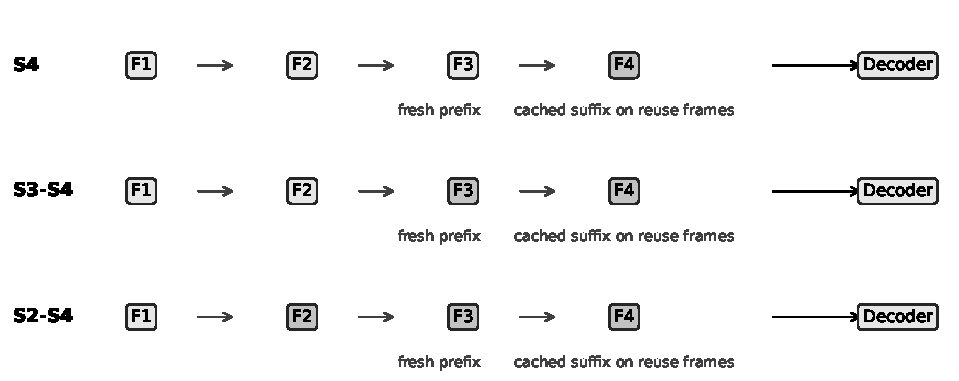
\includegraphics[width=\columnwidth]{method_overview.pdf}
  \caption{The three controlled reuse boundaries. The fresh prefix changes with the boundary; the cached suffix is reused on non-refresh frames and the decoder remains active.}
  \label{fig:method}
\end{figure}

\subsection{Refresh interval and three analytical levels}
FI-2, FI-4, and FI-8 refresh every second, fourth, and eighth frame respectively, subject to the compulsory first refresh in each video. We report the actual refresh fraction because video boundaries make it slightly larger than the nominal ratio. The study distinguishes three levels: (i) \emph{semantic tolerance}, measured by validation mIoU drop under stale features; (ii) \emph{computational opportunity}, measured by stage calls and profiled removable suffix runtime; and (iii) \emph{realized hardware benefit}, measured by paired CUDA input-to-logits latency. Algorithmic computation avoidance therefore need not imply proportional wall-clock acceleration.

\section{Experimental Protocol}
\subsection{Dataset and frozen models}
We use the official VSPW validation split \cite{miao2021vspw}: 343 videos, 24,392 RGB/ground-truth pairs, 124 classes, and ignore label 255. The reported values are validation-system results rather than independent public test results. We evaluate frozen VSPW-compatible SegFormer-B0 and B1 checkpoints; no model, data split, or training procedure is changed in this round.

\subsection{Boundary and timing matrix}
The matrix contains Full plus nine reuse settings per model: three boundaries crossed with FI-2/FI-4/FI-8. Stage 1--3 remain fresh for S4, Stage 1--2 remain fresh for S3--S4, and Stage 1 remains fresh for S2--S4. The decoder runs on every frame. Physical stage-call counters record the omitted work, and persistent feature memory is audited separately as logical cache versus allocated cache.

Table~\ref{tab:calls} gives a concrete physical-execution check for FI-8. The same counter pattern holds for FI-2 and FI-4, with the refresh-frame counts changing according to the interval. These counters are collected from the forward modules rather than inferred from the nominal schedule; thus a cached suffix contributes no stage call on a reuse frame.

\begin{table}[t]
\centering
\caption{Physical calls over the 24,392-frame validation sequence at FI-8. The pattern is identical for B0 and B1.}
\label{tab:calls}
\scriptsize
\setlength{\tabcolsep}{2.5pt}
\begin{tabular}{lrrr}
\toprule
Boundary & Fresh-stage calls & Cached-suffix calls & Decoder calls \\
\midrule
Full & S1--S4: 24,392 each & none & 24,392 \\
S4 & S1--S3: 24,392 each & S4: 3,181 & 24,392 \\
S3--S4 & S1--S2: 24,392 each & S3--S4: 3,181 & 24,392 \\
S2--S4 & S1: 24,392 & S2--S4: 3,181 & 24,392 \\
\bottomrule
\end{tabular}
\end{table}

Latency starts from a CUDA-resident $512\times512$ input tensor and ends when segmentation logits are ready. Measurements use an NVIDIA GeForce RTX 4090 D, PyTorch 2.1.2+cu118, CUDA 11.8, BF16 compute autocast, batch size one, 200 warmup iterations, and 1,000 CUDA-event measurements per repetition. Each configuration has five repetitions and an immediately paired Full baseline in the same process. Video decoding, disk I/O, pageable CPU-to-GPU transfer, visualization, and result writing are excluded.

\section{Results and Analysis}
\subsection{Boundary--interval frontier}
Table~\ref{tab:main} reports all 18 reuse settings. Full validation mIoU is 0.301291 for B0 and 0.371595 for B1. At the conservative S4/FI-2 point, B0 loses 0.091 pp at 1.068$\times$ speedup with CI [1.036,1.100], while B1 loses 0.118 pp at 1.111$\times$ with [1.061,1.200]. The highest-speed settings are S2--S4/FI-8: 2.396$\times$ for B0 with 1.835 pp loss, and 2.282$\times$ for B1 with 2.715 pp loss.

\begin{table*}[t]
\centering
\caption{Complete Round 10 reuse matrix. Refresh is the actual suffix refresh fraction; speedup is the five-repetition paired end-to-end mean with bootstrap 95\% CI.}
\label{tab:main}
\scriptsize
\setlength{\tabcolsep}{3.0pt}
\begin{tabular}{llrrrrrr}
\toprule
Model & Boundary & FI & Refresh (\%) & mIoU drop (pp) & Speedup & CI low & CI high \\
\midrule
B0 & S4 & 2 & 50.381 & 0.091 & 1.068 & 1.036 & 1.100 \\
B0 & S4 & 4 & 25.508 & 0.437 & 1.215 & 1.157 & 1.290 \\
B0 & S4 & 8 & 13.041 & 1.133 & 1.244 & 1.184 & 1.297 \\
B0 & S3--S4 & 2 & 50.381 & 0.184 & 1.254 & 1.220 & 1.286 \\
B0 & S3--S4 & 4 & 25.508 & 0.709 & 1.456 & 1.382 & 1.524 \\
B0 & S3--S4 & 8 & 13.041 & 1.644 & 1.682 & 1.625 & 1.756 \\
B0 & S2--S4 & 2 & 50.381 & 0.231 & 1.505 & 1.390 & 1.621 \\
B0 & S2--S4 & 4 & 25.508 & 0.825 & 2.057 & 2.013 & 2.123 \\
B0 & S2--S4 & 8 & 13.041 & 1.835 & 2.396 & 2.292 & 2.492 \\
\midrule
B1 & S4 & 2 & 50.381 & 0.118 & 1.111 & 1.061 & 1.200 \\
B1 & S4 & 4 & 25.508 & 0.553 & 1.140 & 1.059 & 1.192 \\
B1 & S4 & 8 & 13.041 & 1.435 & 1.181 & 1.139 & 1.228 \\
B1 & S3--S4 & 2 & 50.381 & 0.283 & 1.331 & 1.279 & 1.406 \\
B1 & S3--S4 & 4 & 25.508 & 1.025 & 1.446 & 1.355 & 1.537 \\
B1 & S3--S4 & 8 & 13.041 & 2.335 & 1.659 & 1.613 & 1.731 \\
B1 & S2--S4 & 2 & 50.381 & 0.397 & 1.554 & 1.516 & 1.608 \\
B1 & S2--S4 & 4 & 25.508 & 1.280 & 1.952 & 1.792 & 2.097 \\
B1 & S2--S4 & 8 & 13.041 & 2.715 & 2.282 & 2.086 & 2.479 \\
\bottomrule
\end{tabular}
\end{table*}

The Pareto audit uses mean speedup and mIoU drop, with Full treated as a reference. The same five-point reuse frontier is recovered for both models: S4/FI-2, S3--S4/FI-2, S2--S4/FI-2, S2--S4/FI-4, and S2--S4/FI-8. S4/FI-4 and S4/FI-8 are dominated by earlier-boundary points; S3--S4/FI-4 and FI-8 are also dominated. Under the two tested scales and this GPU, the measured frontier suggests that moving the reuse boundary earlier can be preferable to extending the interval at a later boundary.

\begin{figure}[t]
  \centering
  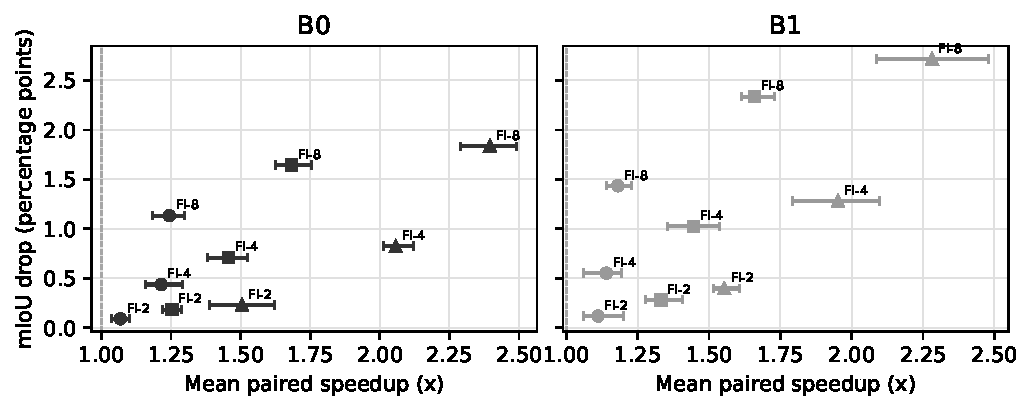
\includegraphics[width=\columnwidth]{round10_boundary_pareto.pdf}
  \caption{Complete boundary--interval speed/quality characterization. Marker shape identifies the reuse boundary; annotations identify the interval.}
  \label{fig:pareto}
\end{figure}

\begin{figure*}[t]
  \centering
  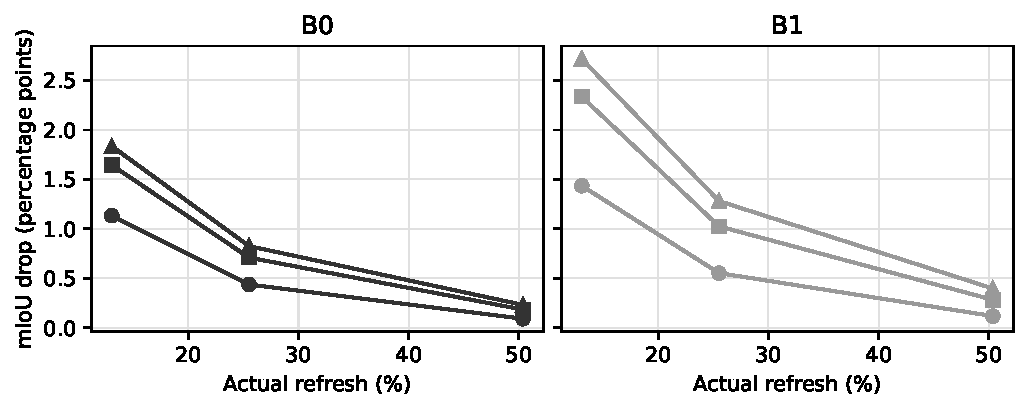
\includegraphics[width=0.82\textwidth]{round10_quality_refresh.pdf}
  \caption{mIoU degradation versus actual refresh fraction for the three boundaries on B0 and B1. Earlier boundaries expose a larger computational suffix but show a steeper quality cost as refresh becomes less frequent.}
  \label{fig:quality}
\end{figure*}

\subsection{Conservative versus aggressive reuse}
S4-only reuse has a distinct conservative operating point relative to the vanilla S3--S4 baseline. For B0, S4/FI-2 gives 1.068$\times$ speedup and 0.091 pp loss, whereas S3--S4/FI-2 gives 1.254$\times$ and 0.184 pp. For B1, the corresponding values are 1.111$\times$/0.118 pp and 1.331$\times$/0.283 pp. S4 does not dominate S3--S4; it occupies a lower-damage point, while S3--S4 exchanges more semantic degradation for more speed. S2--S4/FI-8 is the aggressive speed frontier, not a default policy.

\subsection{Pareto ordering across model scale}
The complete dominance audit recovers the same five-point frontier for both model scales, but the numerical trade-off is not identical. At FI-2, moving from S4 to S3--S4 increases speedup by 0.186$\times$ for B0 and 0.220$\times$ for B1, while increasing mIoU loss by 0.093 and 0.165 pp, respectively. Moving to S2--S4/FI-2 gives 1.505$\times$/0.231 pp for B0 and 1.554$\times$/0.397 pp for B1. At the aggressive endpoint, B1 retains a smaller speedup than B0 but incurs a larger quality loss. This is a model-scale comparison under a fixed protocol, not evidence of a scale-independent law.

\subsection{Runtime opportunity and realized speed}
Table~\ref{tab:profile} shows similar suffix composition across model scale. S4 accounts for 18.42\% and 18.54\% of profiled B0/B1 full runtime; cumulative S3--S4 and S2--S4 shares are 41.45\%/42.29\% and 64.12\%/64.81\%. The earlier boundary therefore exposes more removable runtime, but the measured speedup also includes the fresh prefix, the always-active decoder, cache control, and GPU kernel behavior. The relationship is directional rather than proportional.

\begin{table}[t]
\centering
\caption{Profiled cumulative suffix opportunity and corrected cache audit. Logical cache is boundary-specific; allocated cache is the actual F2--F4 state retained by the current implementation.}
\label{tab:profile}
\scriptsize
\setlength{\tabcolsep}{2.2pt}
\begin{tabular}{lrrrrrr}
\toprule
Model & S4 & S3--S4 & S2--S4 & Log. S4 & Log. S3--S4 & Log. S2--S4 \\
 & \multicolumn{3}{c}{runtime share (\%)} & \multicolumn{3}{c}{cache (MiB)} \\
\midrule
B0 & 18.42 & 41.45 & 64.12 & .250 & .875 & 1.875 \\
B1 & 18.54 & 42.29 & 64.81 & .500 & 1.750 & 3.750 \\
\bottomrule
\end{tabular}
\\[-2pt]
\scriptsize Allocated persistent cache: B0 1.875 MiB; B1 3.750 MiB.
\end{table}

\begin{figure}[t]
  \centering
  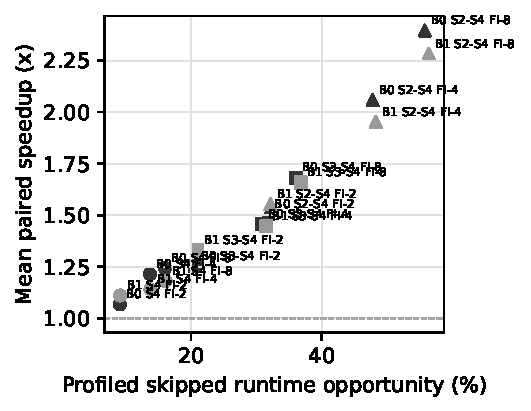
\includegraphics[width=\columnwidth]{round10_runtime_opportunity.pdf}
  \caption{Profiled skipped-runtime opportunity versus paired speedup, using only Round 10 RTX 4090 D measurements.}
  \label{fig:runtime}
\end{figure}

\subsection{Correctness, scale, and limitations}
The 100\% refresh equivalence gate passes for B0 and B1 at all three boundaries on 20 real validation frames, with maximum absolute error, mean absolute error, and relative L2 equal to zero. This verifies the refresh and cache plumbing; it does not claim that a reused feature equals the current-frame feature. Physical call counters provide the complementary compute proof: at FI-8, S4 executes Stage 4 on 3,181 of 24,392 frames, S3--S4 executes Stages 3--4 on those frames, and S2--S4 executes Stages 2--4 on those frames, while the decoder executes on all frames.

The lowest-damage boundary and highest-speed boundary are stable across B0 and B1, and the audited five-point frontier is reproduced across scale. The scope is limited to one VSPW validation split, one GPU model, two SegFormer scales, fixed intervals, and no cross-architecture or edge-device validation. No dynamic scheduler, adaptive selector, TensorRT, ONNX, or custom kernel is evaluated. Earlier fine-grained partial computation is omitted from the quantitative tables because its historical RTX 4090 protocol is separately scoped and not comparable to these RTX 4090 D measurements.

The paired timing design also limits a common source of optimism in reuse studies. Every reuse setting is compared with an immediately measured Full baseline in the same process, and the reported intervals are bootstrap intervals over five paired repetitions. The conservative points remain distinguishable from unity in the measured means: B0 S4/FI-2 is 1.068$\times$ with CI [1.036,1.100], and B1 S4/FI-2 is 1.111$\times$ with CI [1.061,1.200]. The aggressive endpoints are larger, but their quality costs are also larger. These intervals describe this repeated GPU protocol; they are not a portability guarantee across devices or software stacks.

Cache accounting separates the memory logically required by a boundary from the tensors retained by the implementation. With FP32 persistent outputs, logical cache is 0.250/0.875/1.875 MiB for S4/S3--S4/S2--S4 on B0 and 0.500/1.750/3.750 MiB on B1. The current pipeline retains all F2--F4 tensors after refresh, so its allocated persistent cache is 1.875 MiB for B0 and 3.750 MiB for B1 even when a shallower boundary uses only F4. Reporting both values avoids treating an implementation allocation detail as a boundary property.

The study has four deliberate limits. It uses the VSPW validation split rather than a held-out cross-dataset test, fixes the input resolution and batch size, evaluates only SegFormer-B0/B1, and measures one RTX 4090 D software stack. It therefore establishes a reproducible boundary characterization, not a universal scheduler or hardware model. The evidence also covers whole-stage dense reuse only; finer-grained token or block reuse is outside the present claim boundary.

\section{Conclusion}
This paper isolates where temporal feature reuse is placed inside a hierarchical segmentation Transformer and measures what survives real GPU execution. Whole-stage reuse yields a clear boundary-dependent frontier: S4/FI-2 is the conservative low-damage point, while S2--S4/FI-8 is the speed frontier. The ordering is reproduced on SegFormer-B0 and B1, but the exact gain is shaped by fresh computation, decoder cost, cache allocation, and GPU behavior. The resulting claim is deliberately bounded: under the tested VSPW validation protocol and RTX 4090 D, semantic tolerance, physically skipped stages, and measured latency must be considered jointly when selecting a temporal reuse boundary.

\clearpage
\bibliographystyle{IEEEbib}
\bibliography{references}

\end{document}
